%% This is an example first chapter.  You should put chapter/appendix that you
%% write into a separate file, and add a line \include{yourfilename} to
%% main.tex, where `yourfilename.tex' is the name of the chapter/appendix file.
%% You can process specific files by typing their names in at the 
%% \files=
%% prompt when you run the file main.tex through LaTeX.
\chapter{Project Management}

\section{Planning}

The project started on September 2013 with full-time dedication on it was planned to be finished by the 2th of December 2013. The first steps were to study its feasibility in terms of technology, to outline the vision and specify the requirements with CREAF. Next steps included the design and implementation of the identified major components of the solution. It would end with the infrastructure setup, testing and the writing of the current document.

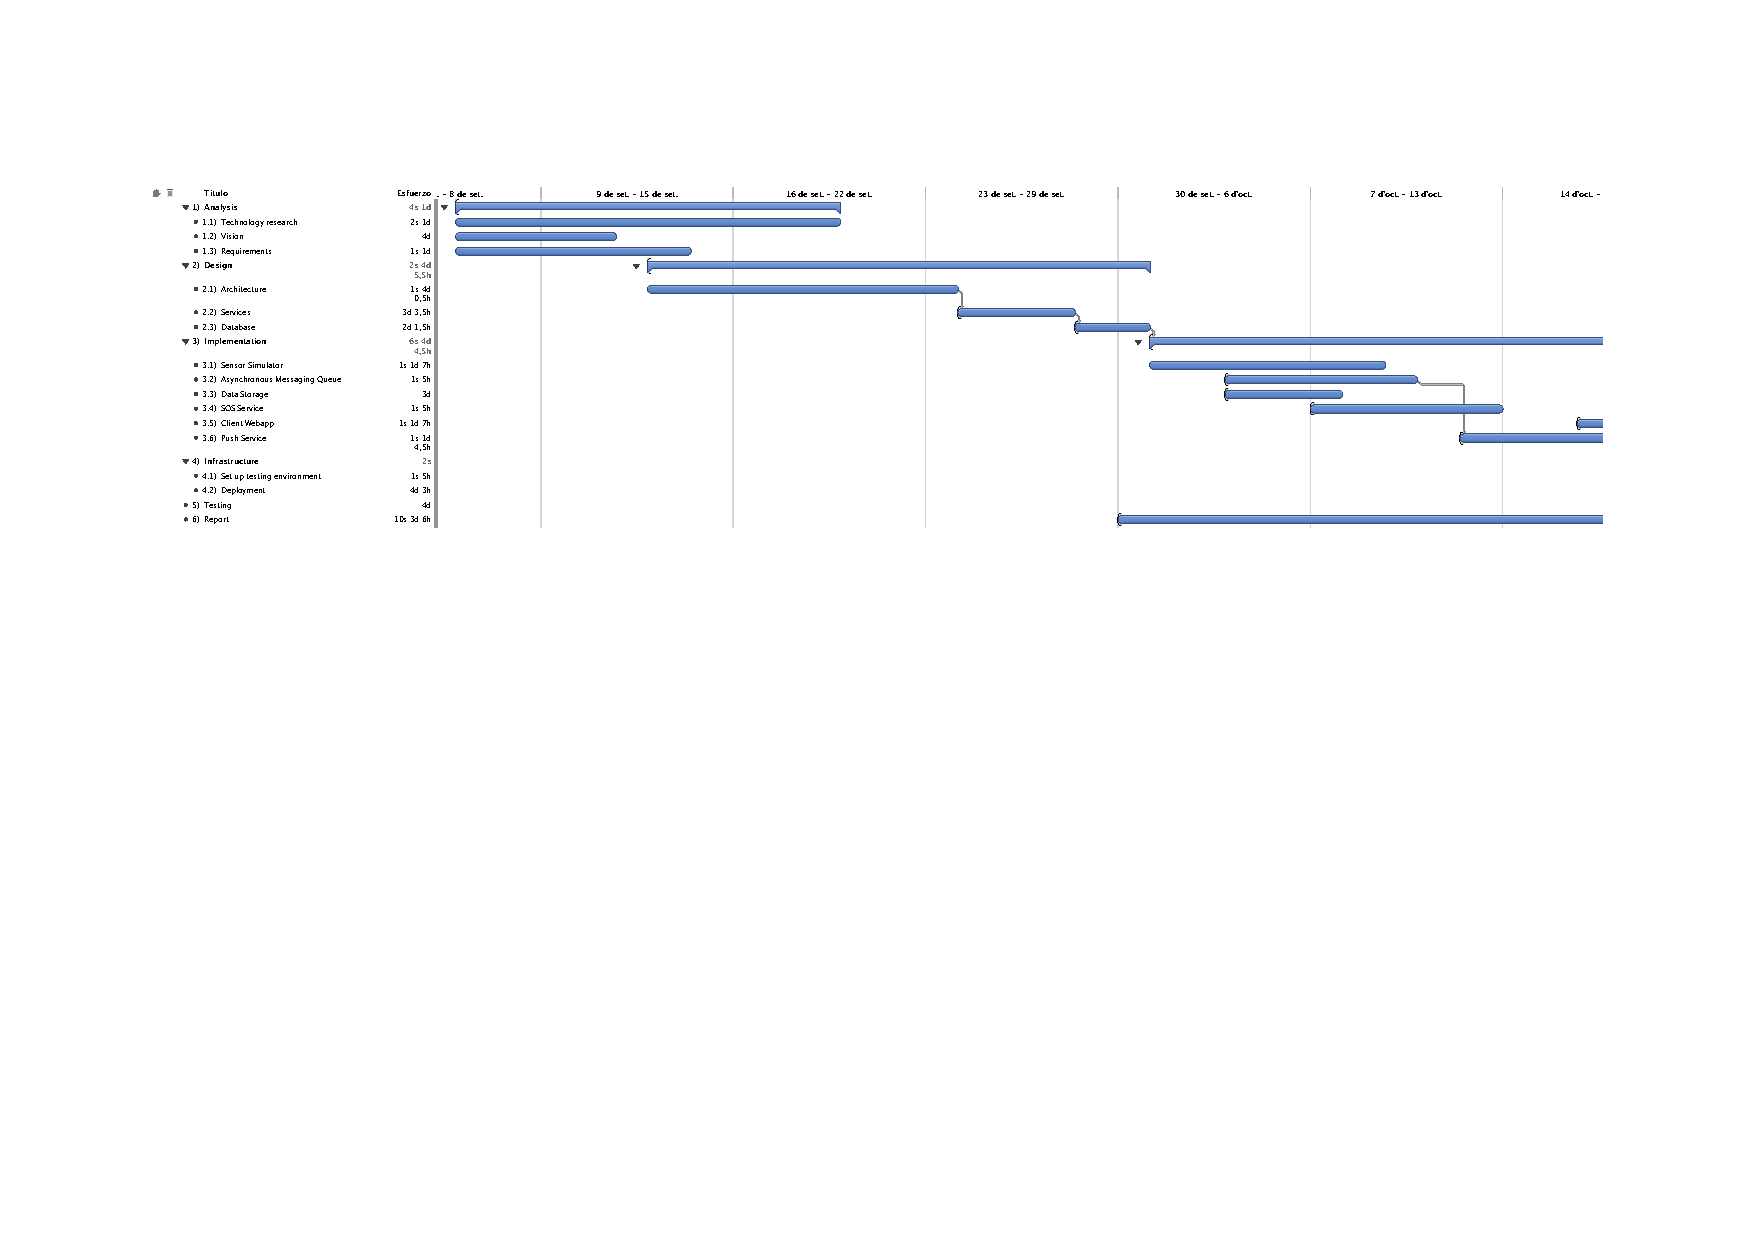
\includepdf[landscape=true, pages={1-2}]{initial_planning}

\section{Cost}

The human resources involved in the project must be considered in order to forecast the costs of the project. These are an analyst, who will be in charge of the Analysis and Design, a Developer, who will implement the design and a System administrator, who will set up the infrastructure.

Regarding the infrastructure, as it relies only on AWS free tier it will not incur in any cost. Therefore, considering these human resources and the initial planning the overall cost is $15250\euro{}$, as detailed below.

\begin{table}[H]
    \centering
    \begin{tabular}{|l|c|c|r|}
    \hline
    \textbf{Resource}  & \textbf{Cost/Hour}  & \textbf{Hours}  & \textbf{Cost} \\ \hline
    Analyst            & 40\euro{}/h         & 200             & 8000\euro{}   \\ \hline
    Developer          & 25\euro{}/h         & 250             & 6250\euro{}   \\ \hline
    SysAdmin           & 20\euro{}/h         & 50              & 1000\euro{}    \\ \hline
    \textbf{Overall}   &                     &                 & \textbf{15250\euro{}} \\ \hline
    \end{tabular}
    \caption{Budget}
    \label{tab:budget}
\end{table}

Besides the time spent on the different stages of the development, additional time must be considered in order to write the current document. To that end, 90 additional hours plus the $200h + 250h + 45h = 495h$ invested by these human resources must be allocated, totalling $495h + 100h = 600h$.

\section{Execution}

Unfortunately, the initial planning has suffered few setbacks during its execution. It was first delayed by the beginning of December by the need of finding a job and the time spent working on a technical test required for a job offer. The major delay was caused by the impact the full-time job had in the dedication time, causing to nearly stop the project during some weeks. Slightly      reactivated working on it occasionally, it was not until allocating 2 hours every day and full-time dedication during weekends that it took off effectively. As a consequence, the planning for the remaining tasks was defined as follows.

Regarding the cost, AWS free tier provided not to be enough to fulfil the needs of the required infrastructure. Using three servers exceeded the maximum of 750 hours of EC2 micro instance usage. The overall cost has been 20.27\$ so far, missing the cost for June 2014.

Moreover, while executing this final planning, another delay was encountered. A disproportionately large Amazon AWS bill was received for what look like an either attack to the system or a billing error. This required to shut the infrastructure down until the issue was resolved. Although having some impact, fortunately it didn't affect much the planning.

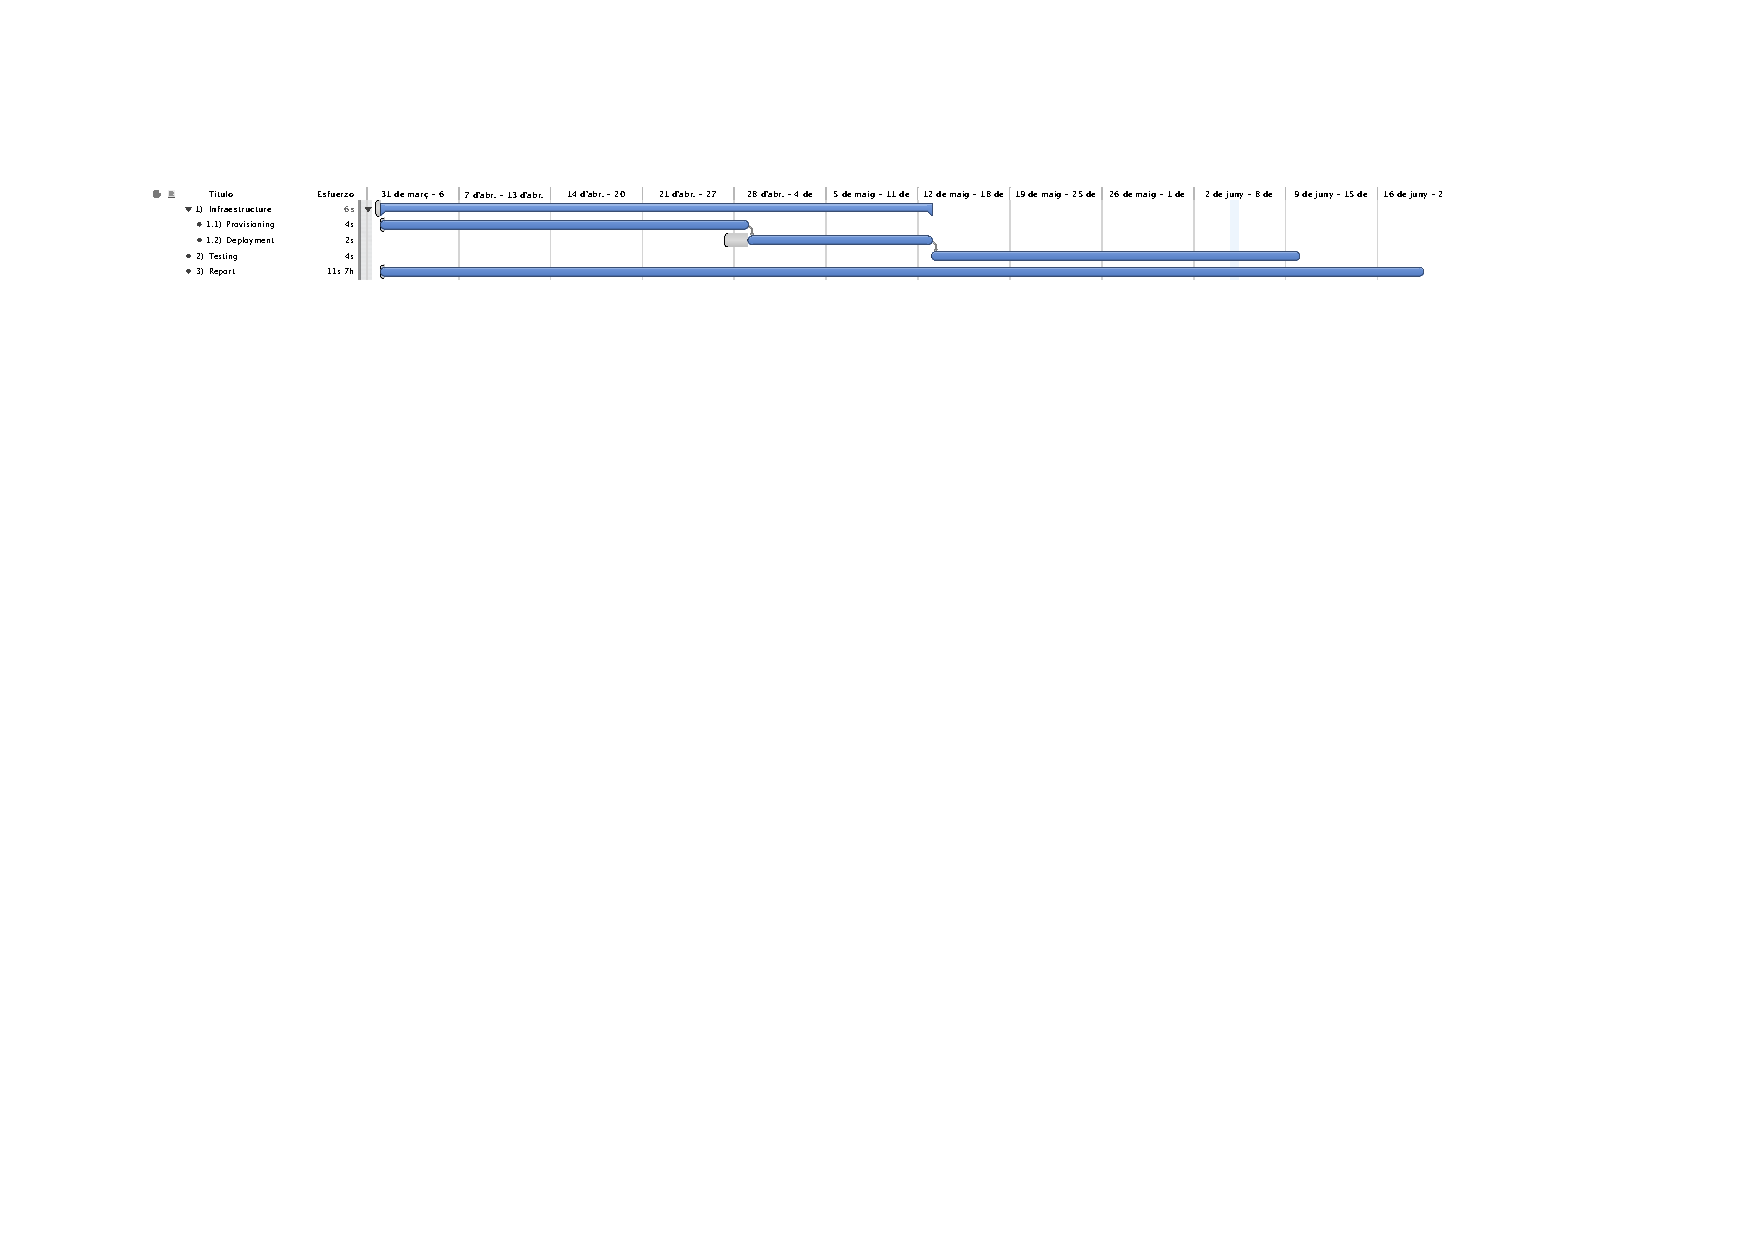
\includepdf[landscape=true, pages={1-2}]{final_planning}